\section{Energy Calibration}
\label{sec:calibration}

The first step is to calibrate the energy response of the detectors. In order to do so, we will use the photopeaks of the radioactive sources: 1173.84 and 1331.70 keV for $^{60}$Co and 661.65 keV for $^{137}$Cs. The position of the peaks is obtained by fitting the energy spectra with a gaussian fit over a linear background (figs. \ref{fig:calib_Co} and \ref{fig:calib_Cs}), and then averaged across the different distances. 


\begin{figure}[H]
	\begin{minipage}[c]{0.5\linewidth}
	\subfloat[][Channel 0.]{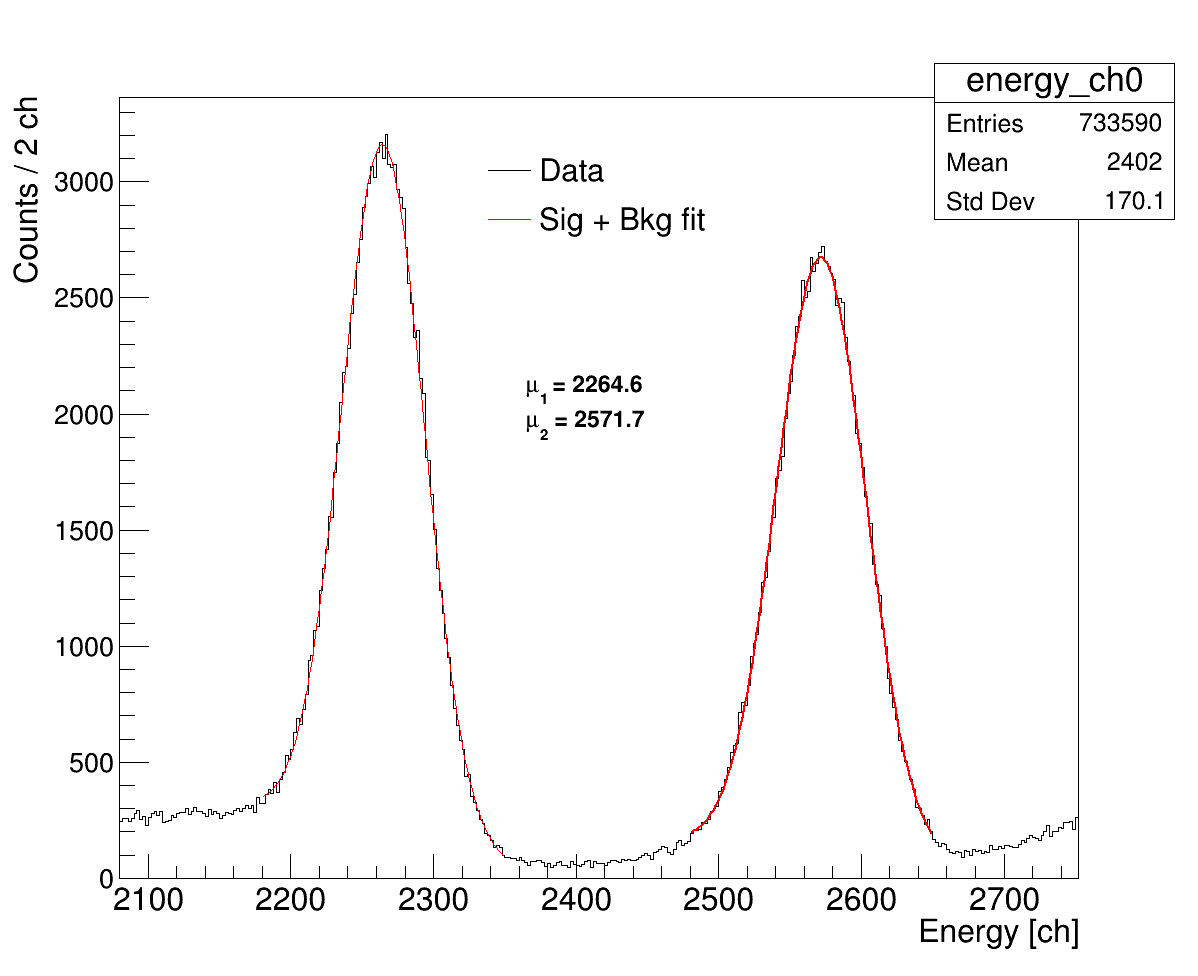
\includegraphics[width=0.9\textwidth]{Images/analysis/calibration/Co10_0.png} \label{fig:calib_Co_0} }
	\end{minipage}
	\begin{minipage}[]{0.5\linewidth}
	\centering
	\subfloat[][Channel 1.]{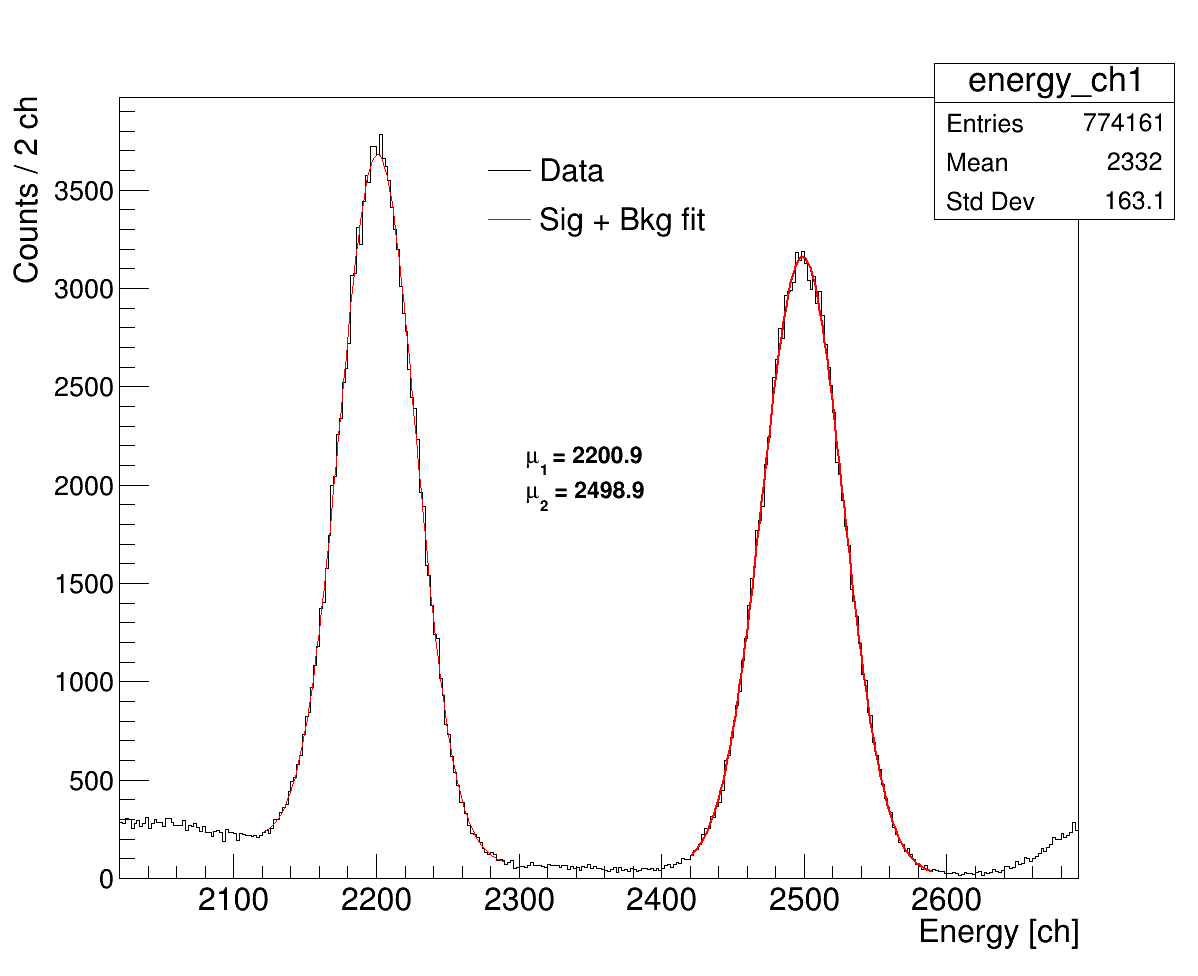
\includegraphics[width=0.9\textwidth]{Images/analysis/calibration/Co10_1.png}  \label{fig:calib_Co_1} }
	\end{minipage}
	\caption{\label{fig:calib_Co} Example of fits for the $^{60}$Co spectra at a distance of 10 cm.}
	\end{figure}


\begin{figure}[H]
	\begin{minipage}[c]{0.5\linewidth}
	\subfloat[][Channel 0.]{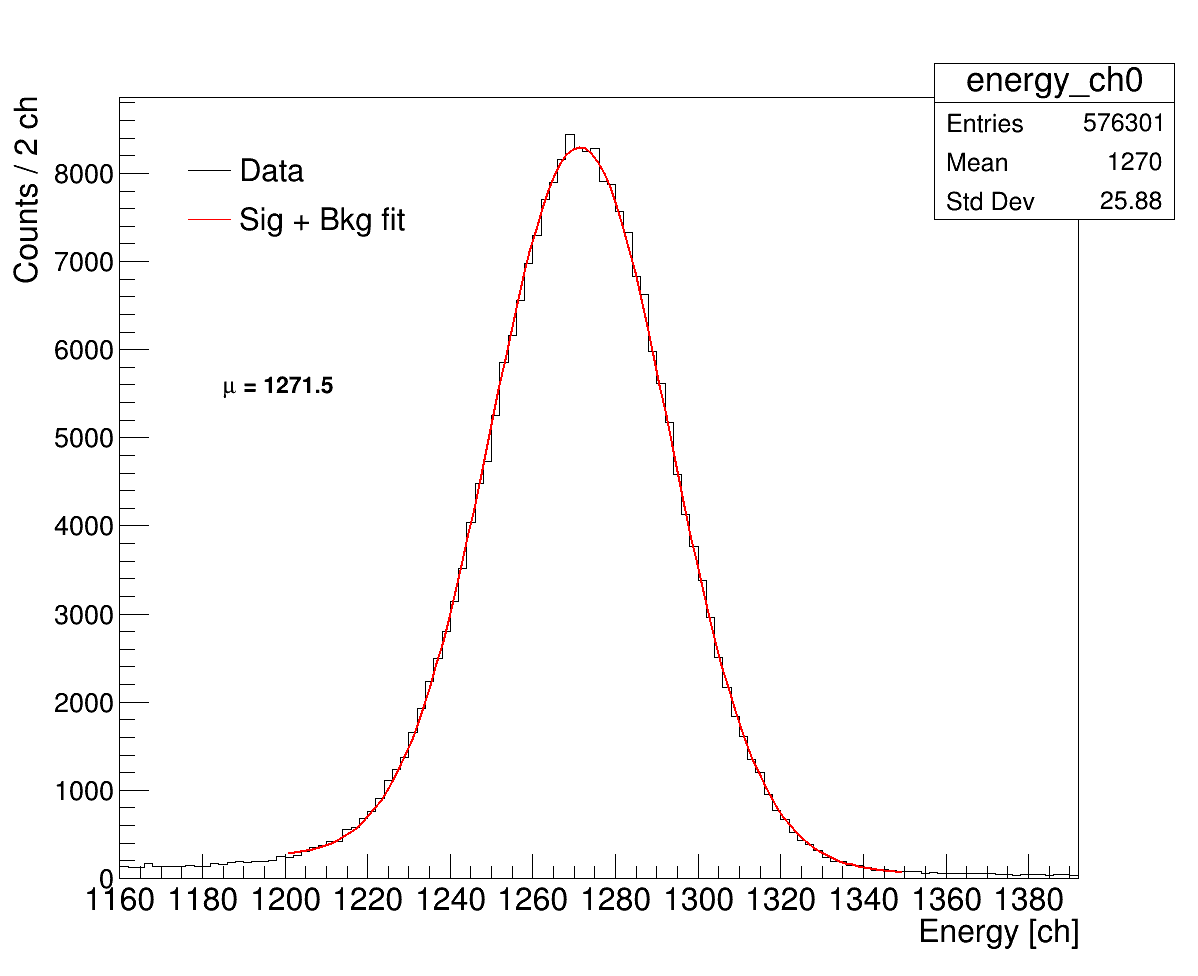
\includegraphics[width=0.9\textwidth]{Images/analysis/calibration/Cs10_0.png} \label{fig:calib_Cs_0} }
	\end{minipage}
	\begin{minipage}[]{0.5\linewidth}
	\centering
	\subfloat[][Channel 1.]{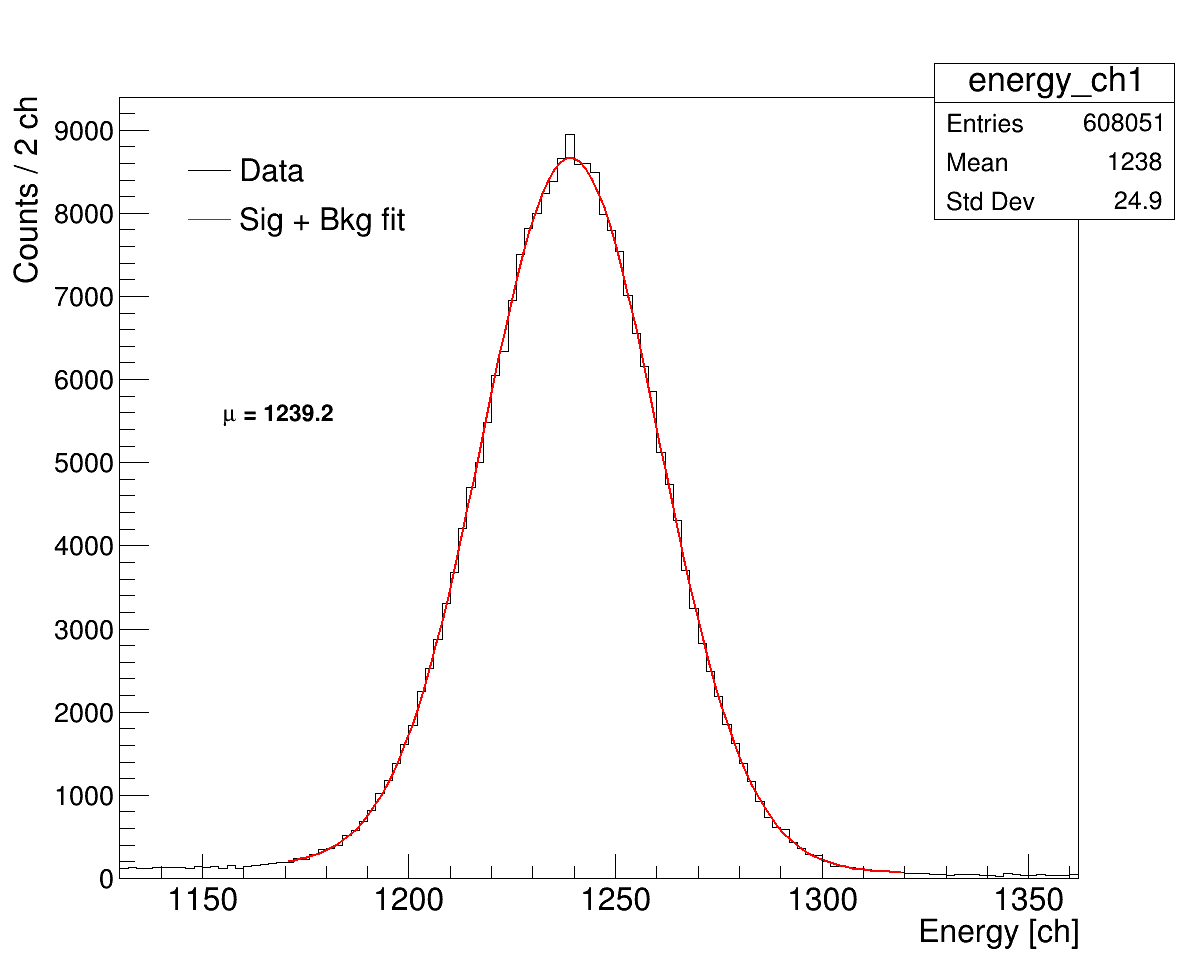
\includegraphics[width=0.9\textwidth]{Images/analysis/calibration/Cs10_1.png}  \label{fig:calib_Cs_1} }
	\end{minipage}
	\caption{\label{fig:calib_Cs} Example of fits for the $^{137}$Cs spectra at a distance of 10 cm.}
	\end{figure}
 

The relationship between energy and read-out channel is given by a linear interpolation of the reference values (fig. \ref{fig:cali}):

\begin{equation}
    E \; \left[keV\right] = m \cdot E \, \left[ch\right] + q
\end{equation}

The resulting values for the two channels are:
\begin{equation}
    \label{eq:calib}
    \begin{align}
        q_0 & = (6.68 \pm 0.05) \; keV \;\;\; 
        m_0   = (0.51785 \pm 0.00003) \; keV \\
        q_1 & = (1.80 \pm 0.04) \; keV \;\;\;
        m_1   = (0.53329 \pm 0.00002) \; keV	
    \end{align}
\end{equation}

\begin{figure}[H]
    \centering
    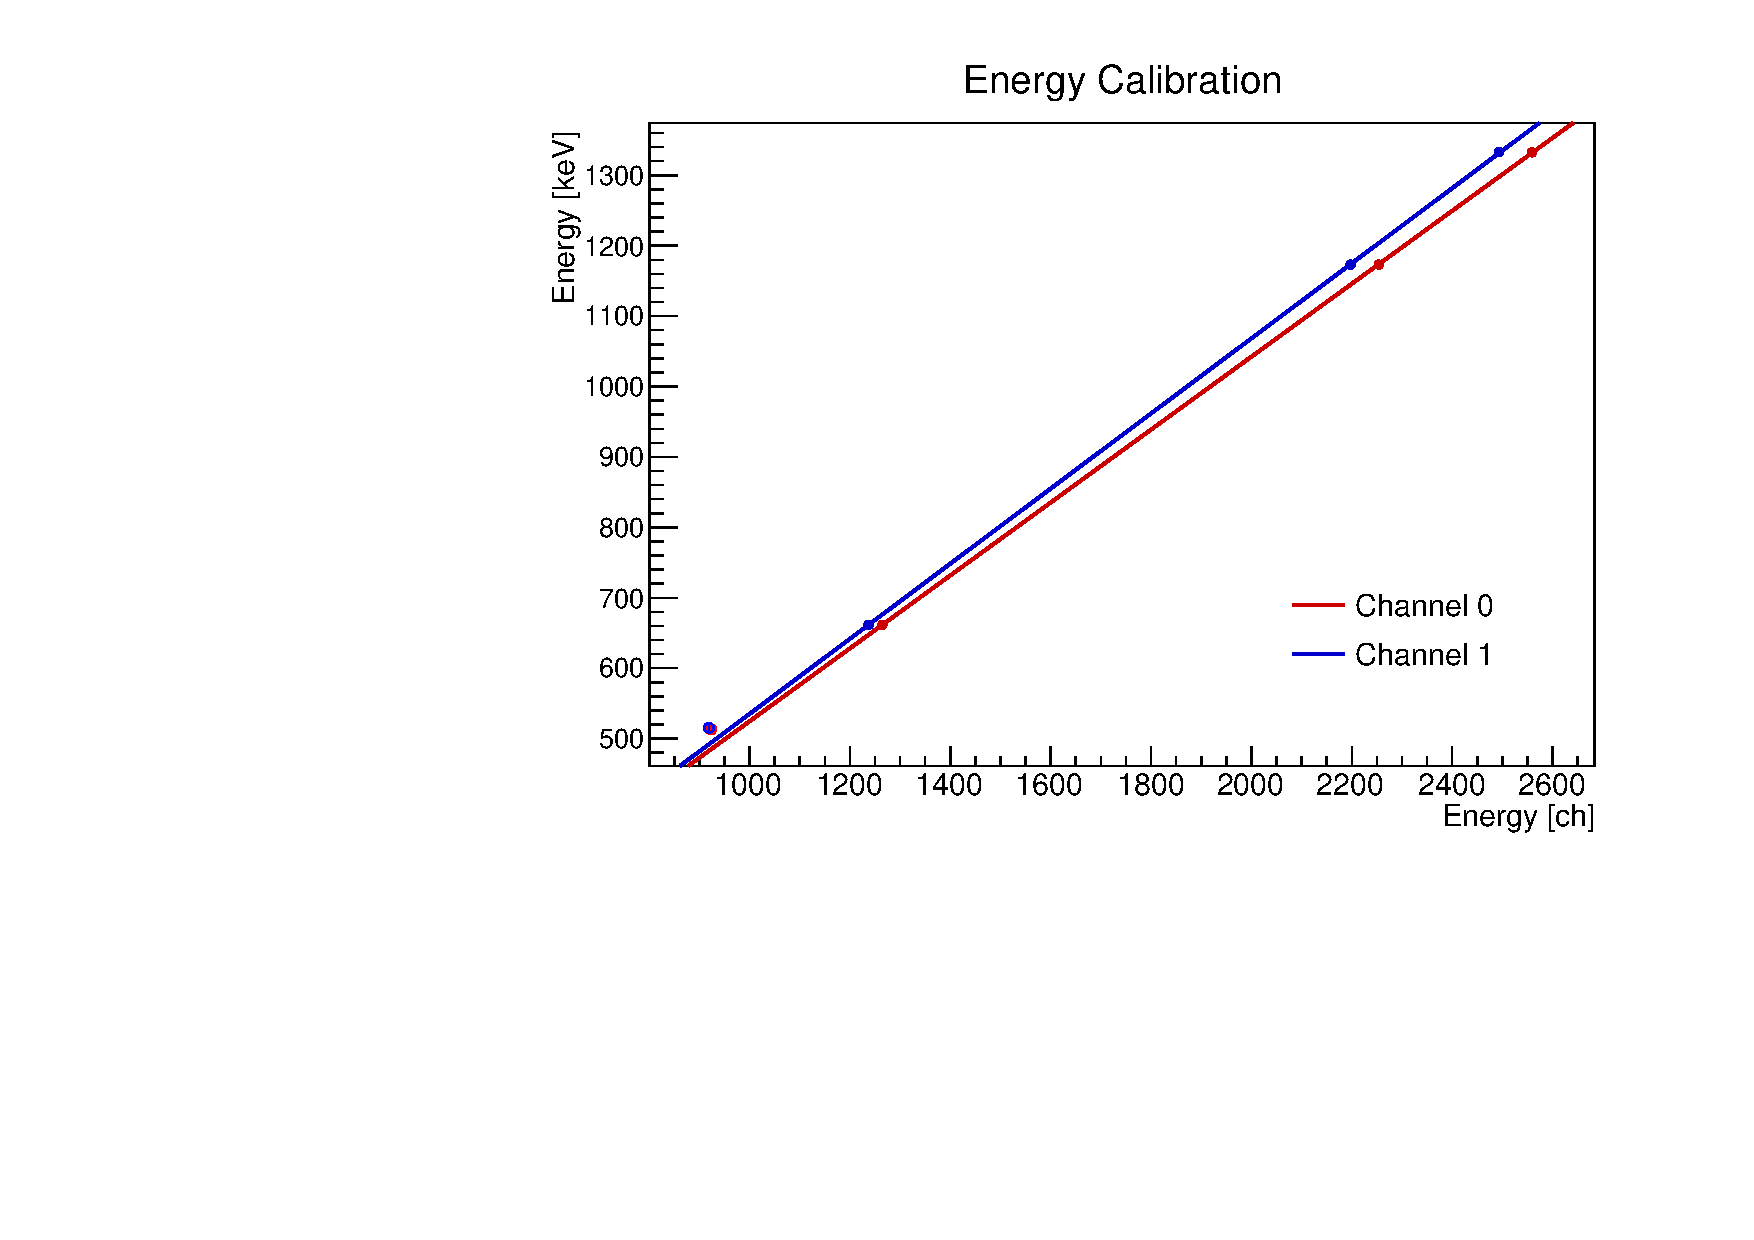
\includegraphics[scale=0.5]{Images/analysis/calibration/cali_2.pdf}
    \caption{Energy calibration of the detectors using $^{60}$Co and $^{137}$Cs, with channel 0 in blue and channel 1 in red. The first point represents for both channels the photopeak of $^{22}$Na at 511 keV, not used for the calibration.}
    \label{fig:cali}
\end{figure}


We then look at the photopeak of $^{22}Na$ at 511 keV. After finding the position as previously explained (fig. \ref{fig:calib_Na}), we can compare the theoretical value to the result expected using the calibration results in eq.\ref{eq:calib}. \\
The difference is of 5.3\% for channel 0 and 3.5\% and 1 respectively. This discrepancy can be due to the fact that the measurements using this source have been conducted on a different day and external factors influenced the calibration, e.g. the crystal temperature. \\
For consistency, we decide to continue using the calibration without $^{22}Na$.


\begin{figure}[H]
	\begin{minipage}[c]{0.5\linewidth}
	\subfloat[][Channel 0.]{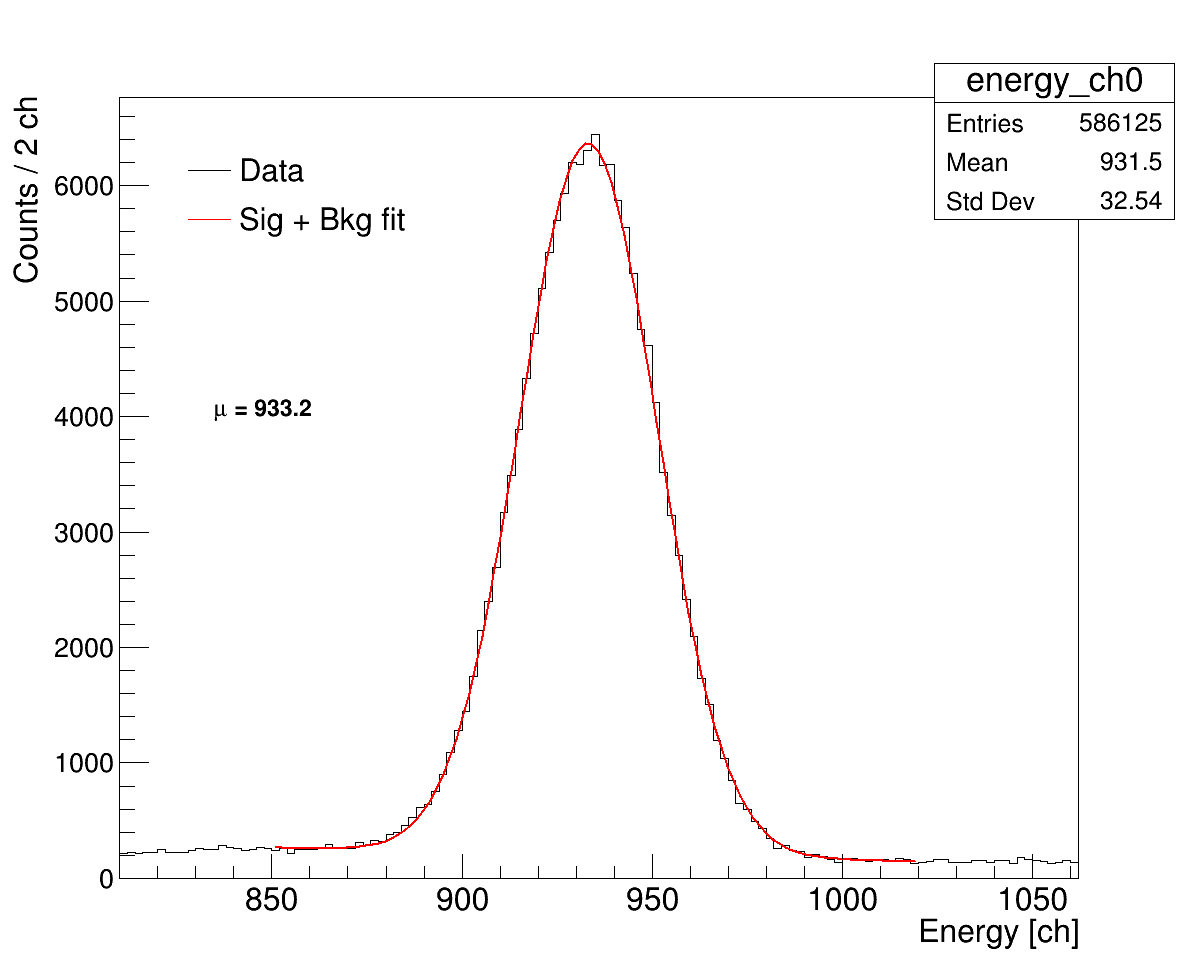
\includegraphics[width=0.9\textwidth]{Images/analysis/calibration/Na10_0.png} \label{fig:calib_Na_0} }
	\end{minipage}
	\begin{minipage}[]{0.5\linewidth}
	\centering
	\subfloat[][Channel 1.]{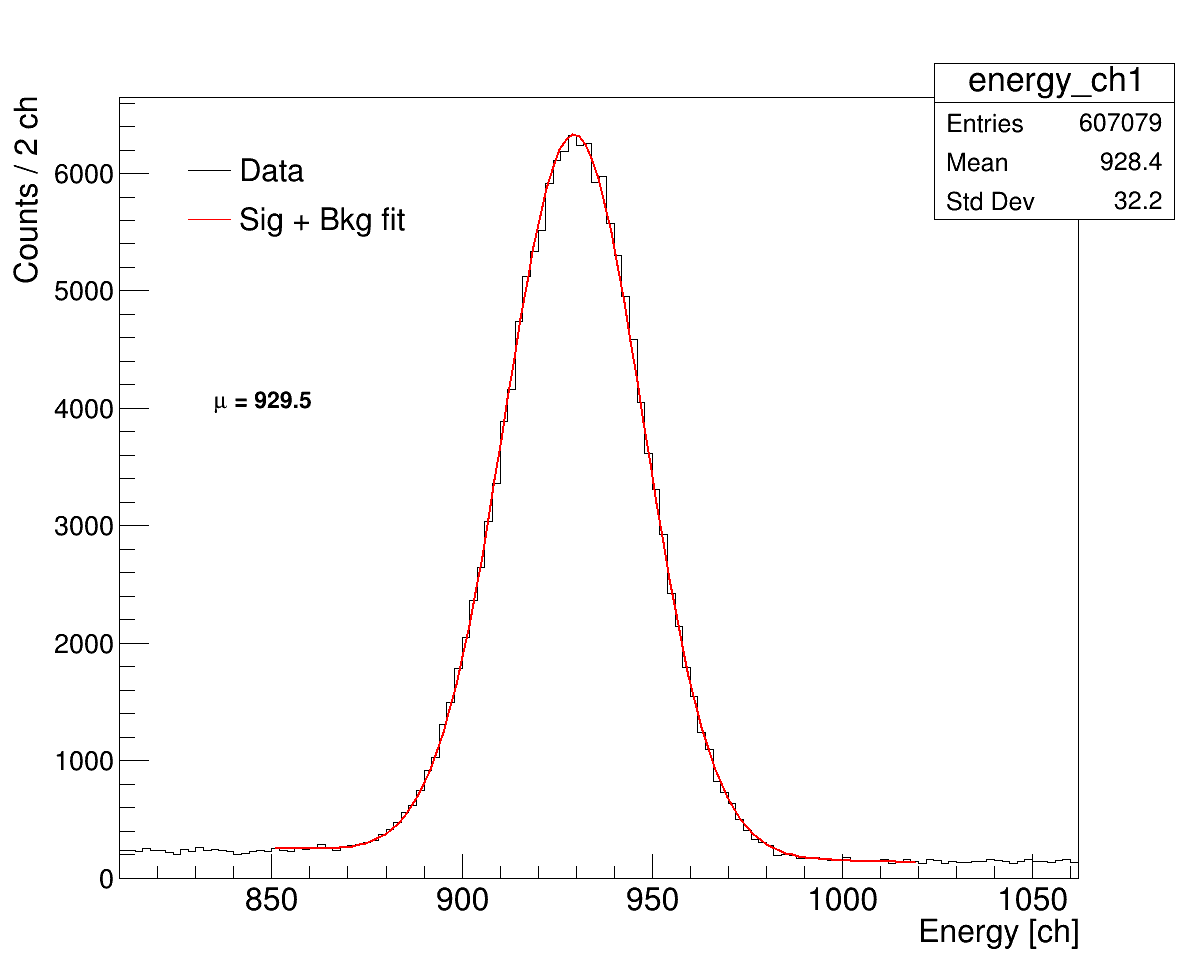
\includegraphics[width=0.9\textwidth]{Images/analysis/calibration/Na10_1.png}  \label{fig:calib_Na_1} }
	\end{minipage}
	\caption{\label{fig:calib_Na} Example of fits for the $^{22}$Na spectra at a distance of 10 cm.}
	\end{figure}





